\chapter{Introduction}
\label{sec:introduction}

To develop this \textbf{Machine Learning} project we are going to use the CRISP-DM methodology, which is a well-known and widely used methodology for data mining projects. It is an iterative process that is composed of six phases.

In particulal, the phases are:
\begin{enumerate}
    \item \textbf{Business Understanding}: in this phase we will try to understand the problem and the objectives of the project. We will also try to understand the data that we have at our disposal and how we can use it to solve the problem.
    \item \textbf{Data Understanding}: in this phase we will try to understand the data that we have at our disposal. We will try to understand the meaning of the data and how we can use it to solve the problem.
    \item \textbf{Data Preparation}: in this phase we will try to prepare the data for the next phases. We will try to clean the data and to transform it in a way that will be useful for the next phases.
    \item \textbf{Modeling}: in this phase we will try to build a model that will be able to solve the problem. We will try to find the best model for our problem.
    \item \textbf{Evaluation}: in this phase we will try to evaluate the model that we have built. We will try to understand if the model is good enough to solve the problem.
    \item \textbf{Deployment}: in this phase we will try to deploy the model that we have built. We will try to understand how we can use the model to solve the problem.
\end{enumerate}

\begin{figure}[H]
    \centering
    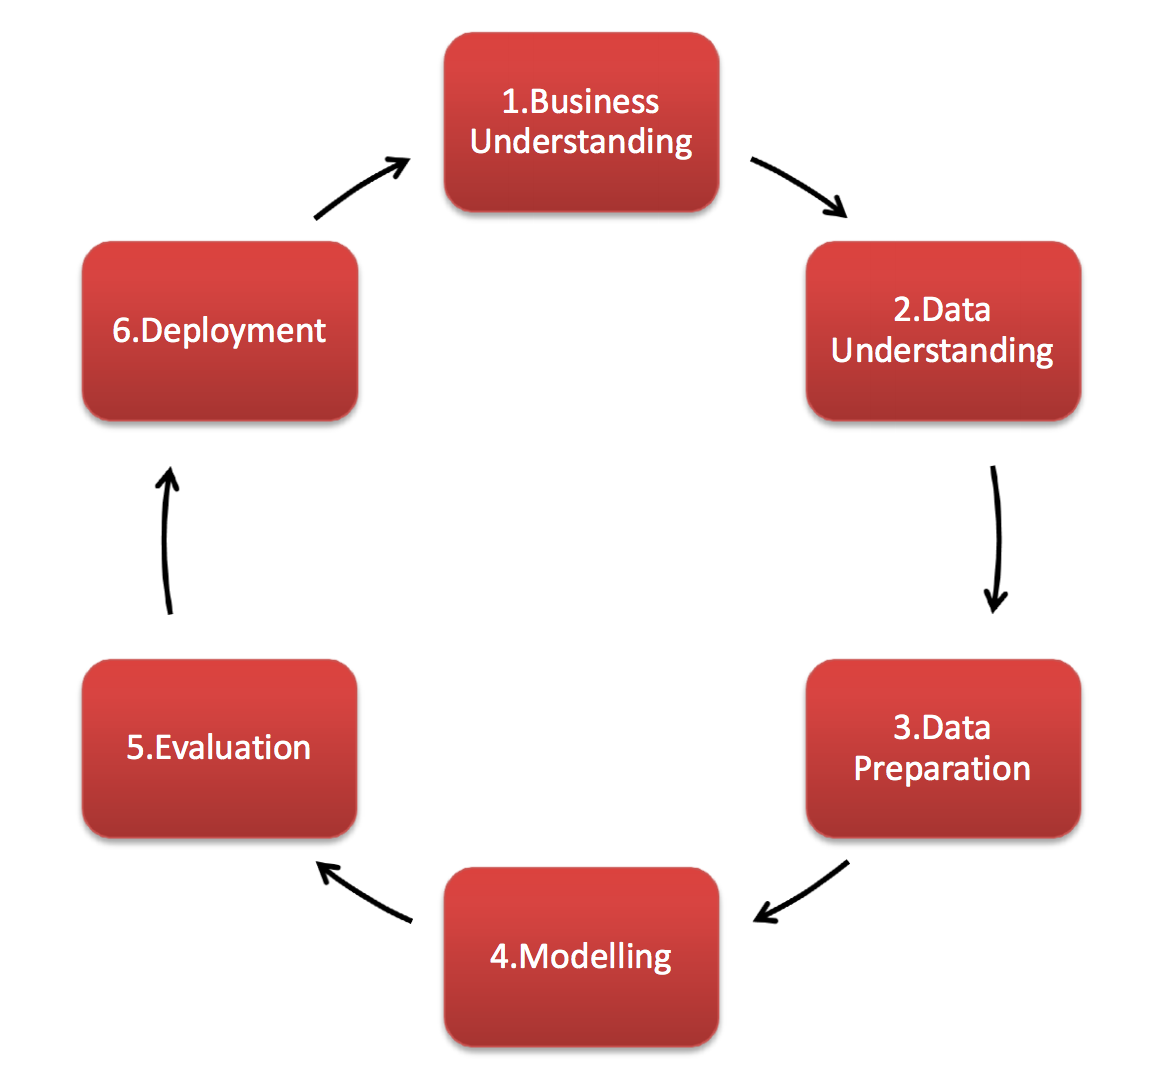
\includegraphics[width=0.5\textwidth]{imgs/crisp.png}
    \caption{CRISP-DM methodology}
    \label{fig:crisp-dm}
\end{figure}
\newpage
